% title: Dead code elimination removes an unused branch
% description: In the example, the used concat contributes to the output and the unused concat does not. DCE removes the unused equation and preserves the output dependency.
\documentclass[tikz,border=5pt]{standalone}
\usetikzlibrary{arrows.meta,shapes.geometric}
\begin{document}
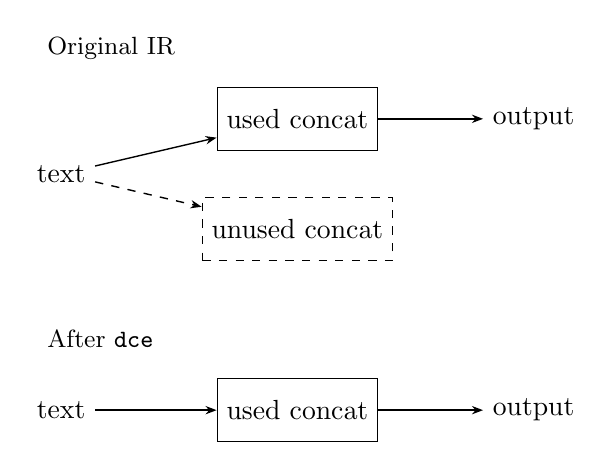
\begin{tikzpicture}[
    box/.style={draw, line width=0.5pt, minimum height=0.8cm,
                minimum width=1.8cm, align=center},
    flow/.style={-{Stealth[length=4pt]}, line width=0.5pt},
    note/.style={font=\small, align=center},
    choice/.style={diamond, draw, line width=0.5pt,
                   aspect=2, inner sep=2pt, align=center},
]

    \node[note,anchor=west] at (-0.3,1.6) {Original IR};
    \node (in) at (0,0) {text};
    \node[box] (used) at (3,0.7) {used concat};
    \node[box,dashed] (unused) at (3,-0.7) {unused concat};
    \node (out) at (6,0.7) {output};
    \draw[flow] (in) -- (used);
    \draw[flow,dashed] (in) -- (unused);
    \draw[flow] (used) -- (out);
    \node[note,anchor=west] at (-0.3,-2.1) {After \texttt{dce}};
    \node (newin) at (0,-3) {text};
    \node[box] (newused) at (3,-3) {used concat};
    \node (newout) at (6,-3) {output};
    \draw[flow] (newin) -- (newused);
    \draw[flow] (newused) -- (newout);

\end{tikzpicture}
\end{document}
